\section{Análisis de riesgos}
\par Es necesario identificar los riesgos para que el gestor del proyecto pueda ir un paso por delante para controlarlos o evitarlos cuando sea posible.
\par Uno de los métodos existentes para identificar los riesgos es crear una lista de comprobación de elementos de riesgo. Esta se puede utilizar para identificar riesgos y se enfoca en un subconjunto de riesgos conocidos y predecibles en las siguientes subcategorías genéricas:

\begin{itemize}[-]
\item \textbf{Tamaño del producto:} riesgos asociados con el tamaño general del software a construir o a modificar.
\item \textbf{Impacto en el negocio:} riesgos asociados con las limitaciones impuestas por la gestión o por el mercado.
\item \textbf{Características del cliente:} riesgos asociados con la sofisticación del cliente y la habilidad del desarrollador para comunicarse con el cliente en los momentos oportunos.
\item \textbf{Tecnología a construir:} riesgos asociados con la complejidad del sistema a construir y la tecnología punta que contiene el sistema.
\item \textbf{Tamaño y experiencia de la plantilla:} riesgos asociados con la experiencia técnica y de proyectos de los ingenieros del software que van a realizar el trabajo.
\end{itemize}

\par Una vez definidas las categorías consideradas, se ha procedido a identificar los riesgos asociados a ellas. Para realizar un análisis objetivo, se ha decidido utilizar una herramienta conocida como Tabla de Impacto. Esta herramienta consiste en una tabla en la que se representa el impacto que tiene cada uno de los riesgos identificados para cuatro objetivos del proyecto (coste, tiempo, alcance y calidad).

\begin{itemize}[-]
\item \textbf{Riesgos del tamaño del producto:}
\begin{itemize}[-]
\item Riesgo-01: Subestimar el tamaño total del proyecto
\begin{table}[h]
\begin{center}
\begin{tabular}{ l l l l l l }
\hline
	 & Muy Bajo & Bajo & Moderado & Alto & Muy Alto \\ \hline \hline
	Coste &  &  &  & X &  \\ \hline
	Tiempo &  &  &  & X &  \\ \hline
	Alcance &  &  &  &  & X \\ \hline
	Calidad &  &  &  &  & X \\ \hline
\end{tabular}
\caption{Riesgo-01.}
\label{Riesgo-01}
\end{center}
\end{table}
\end{itemize}

\item \textbf{Riesgos del impacto en el negocio:}
\begin{itemize}[-]
\item Riesgo-02: La documentación del proyecto elaborada y ofrecida al cliente tiene una calidad insuficiente
\begin{table}[H]
\begin{center}
\begin{tabular}{ l l l l l l }
\hline
	 & Muy Bajo & Bajo & Moderado & Alto & Muy Alto \\ \hline \hline
	Coste &  &  & X &  &  \\ \hline
	Tiempo &  &  & X &  &  \\ \hline
	Alcance & X &  &  &  &  \\ \hline
	Calidad &  &  &  & X &  \\ \hline
\end{tabular}
\caption{Riesgo-02.}
\label{Riesgo-02}
\end{center}
\end{table}
\item Riesgo-03: Costos asociados a un retraso en la entrega
\begin{table}[H]
\begin{center}
\begin{tabular}{ l l l l l l }
\hline
	 & Muy Bajo & Bajo & Moderado & Alto & Muy Alto \\ \hline \hline
	Coste &  &  & X &  &  \\ \hline
	Tiempo &  &  &  & X &  \\ \hline
	Alcance &  &  &  & X &  \\ \hline
	Calidad &  &  & X &  &  \\ \hline
\end{tabular}
\caption{Riesgo-03.}
\label{Riesgo-03}
\end{center}
\end{table}
\end{itemize}

\item \textbf{Riesgos relacionados con el cliente:}
\begin{itemize}[-]
\item Riesgo-04: El cliente no tiene una idea clara de lo que quiere
\begin{table}[H]
\begin{center}
\begin{tabular}{ l l l l l l }
\hline
	 & Muy Bajo & Bajo & Moderado & Alto & Muy Alto \\ \hline \hline
	Coste &  &  &  & X &  \\ \hline
	Tiempo &  &  &  & X &  \\ \hline
	Alcance &  & X &  &  &  \\ \hline
	Calidad &  &  & X &  &  \\ \hline
\end{tabular}
\caption{Riesgo-04.}
\label{Riesgo-04}
\end{center}
\end{table}

\item Riesgo-05: El cliente no entiende el proceso del software
\begin{table}[H]
\begin{center}
\begin{tabular}{ l l l l l l }
\hline
	 & Muy Bajo & Bajo & Moderado & Alto & Muy Alto \\ \hline \hline
	Coste &  &  & X &  &  \\ \hline
	Tiempo &  &  &  & X &  \\ \hline
	Alcance &  & X &  &  &  \\ \hline
	Calidad &  &  & X &  &  \\ \hline
\end{tabular}
\caption{Riesgo-05.}
\label{Riesgo-05}
\end{center}
\end{table}
\end{itemize}

\item \textbf{Riesgos tecnológicos:}
\begin{itemize}[-]
\item Riesgo-06: Falta de experiencia con la tecnología que se pretende utilizar
\begin{table}[H]
\begin{center}
\begin{tabular}{ l l l l l l }
\hline
	 & Muy Bajo & Bajo & Moderado & Alto & Muy Alto \\ \hline \hline
	Coste &  &  &  & X &  \\ \hline
	Tiempo &  &  &  &  & X \\ \hline
	Alcance &  &  &  & X &  \\ \hline
	Calidad &  &  &  & X &  \\ \hline
\end{tabular}
\caption{Riesgo-06.}
\label{Riesgo-06}
\end{center}
\end{table}
\end{itemize}

\item \textbf{Riesgos asociados a la plantilla:}
\begin{itemize}[-]
\item Riesgo-07: Subestimar el número de personas en plantilla requeridas para el proyecto
\begin{table}[H]
\begin{center}
\begin{tabular}{ l l l l l l }
\hline
	 & Muy Bajo & Bajo & Moderado & Alto & Muy Alto \\ \hline \hline
	Coste &  &  &  & X &  \\ \hline
	Tiempo &  &  &  & X &  \\ \hline
	Alcance &  &  & X &  &  \\ \hline
	Calidad &  &  &  & X &  \\ \hline
\end{tabular}
\caption{Riesgo-07.}
\label{Riesgo-07}
\end{center}
\end{table}

\item Riesgo-08: Experiencia o conocimientos del personal insuficientes
\begin{table}[H]
\begin{center}
\begin{tabular}{ l l l l l l }
\hline
	 & Muy Bajo & Bajo & Moderado & Alto & Muy Alto \\ \hline \hline
	Coste &  &  &  & X &  \\ \hline
	Tiempo &  &  &  & X &  \\ \hline
	Alcance &  &  &  & X &  \\ \hline
	Calidad &  &  &  & X &  \\ \hline
\end{tabular}
\caption{Riesgo-08.}
\label{Riesgo-08}
\end{center}
\end{table}
\end{itemize}
\end{itemize}

\subsection{Análisis Cualitativo}
\par Para analizar el impacto real de cada uno de los riesgos identificados, se ha decidido representar su impacto en términos monetarios, así como la probabilidad de que dicho suceso se produjera. Para ello nos hemos basado en las probabilidades mostradas en la tabla que se encuentra a continuación. Este método es conocido como Valor Monetario Esperado (VME).

\begin{figure}[H]
\begin{center}
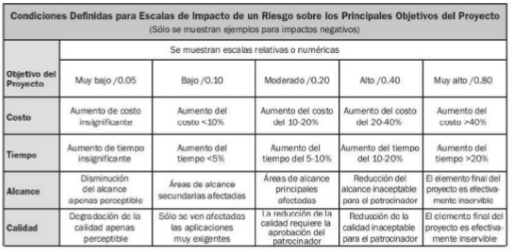
\includegraphics[width=0.5\textwidth]{./img/ImpactoAnalisisCualitativo.png}
\end{center}
\caption{Tabla de Impactos del Análisis Cualitativo}
\label{tab:Tabla de Impactos del Análisis Cualitativo}
\end{figure}

\begin{table}[h]
\begin{center}
\begin{tabular}{ l l l l }
\hline
	Riesgo & Impacto (\euro) & Probabilidad & VME (\euro) \\ \hline \hline
	Riesgo-01 & 3000 & 0.3 & 900 \\ \hline
	Riesgo-02 & 1000 & 0.2 & 200 \\ \hline
	Riesgo-03 & 1500 & 0.3 & 450 \\ \hline
	Riesgo-04 & 2000 & 0.2 & 400 \\ \hline
	Riesgo-05 & 500 & 0.4 & 200 \\ \hline
	Riesgo-06 & 1200 & 0.1 & 120 \\ \hline
	Riesgo-07 & 2500 & 0.2 & 500 \\ \hline
	Riesgo-08 & 5000 & 0.1 & 500 \\ \hline
	Total & 16700 &  & 3270 \\ \hline
\end{tabular}
\caption{Analisis Cualitativo.}
\label{Analisis Cualitativo}
\end{center}
\end{table}

\begin{figure}[H]
\begin{center}
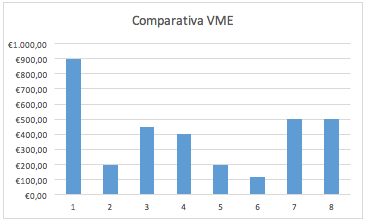
\includegraphics[width=0.5\textwidth]{./img/grafico2.png}
\end{center}
\caption{Grafico análisis cualitativo}
\label{tab:Grafico análisis cualitativo}
\end{figure}
